\documentclass[11pt,noanswers,addpoints]{exam}
%\documentclass[11pt,letter]{article}
\usepackage{pslatex}
\usepackage{helvet}
\renewcommand*\familydefault{\sfdefault} % Use the sans serif version of the font

\usepackage[pdftex]{graphicx}
\usepackage{amsmath}
\usepackage{amssymb}
\usepackage[margin=0.5in,bottom=1in]{geometry}

%\usepackage[left=1in,right=1in,top=0.7in,bottom=1in]{geometry}
\usepackage{booktabs}
\usepackage{url}

\usepackage{listings}% http://ctan.org/pkg/listings
\lstset{
  basicstyle=\ttfamily,
  mathescape
}

\setlength\parindent{0pt}


\newcommand\note[1]{\textcolor{red}{#1}}
\begin{document}

{\Large{\textbf{Machine Learning}}} \\[2mm]
\textbf{\Huge{Lab 2: Density estimation}}\\[2mm]
%{T 04:00pm--05:00pm, Wilson Hall 1-144}\\[2mm]


\section{Overview}
In this lab we will consider the problem of estimating, using a collection of observations, 
the probability of generating a particular future observation. You will use two approaches to
this problem: parametric and non-parametric density estimation.

In the former case, you will look at the salaries for employees of the city of Chicago. Assuming
that the salaries within each department are sampled from a Gaussian distribution, you will learn the
underlying model. The second data set we will consider is crime in the same city. You will generate a crime 
``heat map" of the city for different types of crimes and in different years to better understand where, and when,
crime takes place. All data used here is publicly available at \texttt{data.cityofchicago.org}.

\section{Provided Resources}


\begin{itemize}
\item \texttt{gaussfit.m} - A placeholder function which will learn the parameters for a Gaussian density function
fit to the provided data.
\item \texttt{kde.m} - A placeholder function which will evaluate the density function for data using Gaussian kernel 
density estimation.
\item \texttt{kdemap.m} - Helper function which calls $\texttt{kde.m}$ in order to generate a map of crime over the 
city of Chicago. For example, $\texttt{imagesc(kdemap(lat, lon, 0.01, 100))}$ will return a 100-by-100 entry grid
sampling of the kernel density estimate using all crimes and a Gaussian kernel of standard deviation $0.01$. Note that
there are over 5 million crimes, so don't expect to be able to run this using all the data.
\item \texttt{crimes.mat} - Data file containing crimes in the city of Chicago with latitude, longitude, and 
the type of crime. Contains: \texttt{lat} and \texttt{lon} - The latitude and longitude of each of 5.6 million crimes.
\texttt{type} - For each crime, which category it falls into. \texttt{year} - The year in which each crime took place.
\texttt{types} - Text names for each type of crime, and the index it corresponds with.
\item \texttt{employees.mat} - Data file containing the salaries for employees of the city of Chicago,
along with the department in which they work. Contains: \texttt{dept} - integers indicating the department
for which each employee works, one for 32,160 total employees. \texttt{depts} - a struct which has text names
for each of 35 departments. \texttt{sal} - the annual salary in dollars for each employee.
\end{itemize}

\section{Guide}

\subsection{Gaussian MLE}
Consider a multivariate Gaussian distribution with \emph{isotropic} covariance matrix, $\Sigma=\sigma^2 I$. 
Note its expression is derived from the standard multivariate Gaussian distribution by assuming isometric covariance.

For a collection of i.i.d. data points $x_i$, the joint probability is computed as the product of individual probabilities:
$$\prod_i \frac{1}{(2\pi\sigma^2)^{D/2}} e^{-\frac{||x_i - \mu||_2^2}{2\sigma^2}}.$$

Given a data set, the \emph{maximum likelihood estimators} for this distribution can be worked out exactly, and the solution is given by
$$\hat{\mu} = \frac{1}{N} \sum_i x_i$$
and
$$\hat{\sigma} = \sqrt{\frac{1}{DN} \sum_i||x_i - \hat{\mu}||_2^2}.$$

\begin{enumerate}
\item Complete and turn in the function \texttt{gaussfit.m}. This function should learn the maximum likelihood estimates for  mean $\mu$ and variance $\sigma^2$ of a collection
of data points, assuming the isotropic Gaussian model, above.
\item Load the file \texttt{employees.mat} containing employee salaries and their respective department
assignment. 
\item For each department use \texttt{gaussfit.m} to learn the parameters of the assumed underlying Gaussian
distribution (in this case, the observation space is 1D). Hint: the salaries for individuals only in the health department
(number 13) can be found using \texttt{sal(dept == 13)}.
\item  Which departments have salary distributions with the highest and lowest mean salary? 
\item  Which departments have the greatest and least variance in salary? Anything special happening?
%\item  Which departments are most and least likely to ``pay" someone -\$10,000 a year? For this you will need to compute the value of 
% the Gaussian probability distribution at $-10,000$ using the parameters you have learned.
\end{enumerate}

\subsection{Kernel density estimation}
\begin{enumerate}
\item  Complete and turn in the function \texttt{kde.m}. This uses kernel density estimation with a Gaussian kernel of
given standard deviation to sample an estimated probability distribution. Given the $N$ observation vectors $x_i$ and a
standard deviation $\sigma$, this function should calculate for each sampling point $z$ the quantity

$$p(z) = \frac1N \sum_{i=1}^N \frac{1}{(2\pi\sigma^2)^{D/2}}\text{exp}\left(-\frac{||x_i - z||_2^2}{2\sigma^2}\right).$$

\item Load the file \texttt{crimes.mat} containing years of criminal activity in the city of Chicago.
\item Using the helper function $\texttt{kdemap.m}$, test your code by generating a heatmap of gambling crimes (crime index
15) for the year 2014 with Gaussian kernels of standard deviation $\sigma = 0.01$. The latitude of
 these crimes can be found for example using $\texttt{lat(type == 15 \& year == 2014)}$ (similarly for longitude). Your result should look similar to this
 (the approximate city boundary was added here to demonstrate the region shown by \texttt{kdemap.m}):
\begin{center}
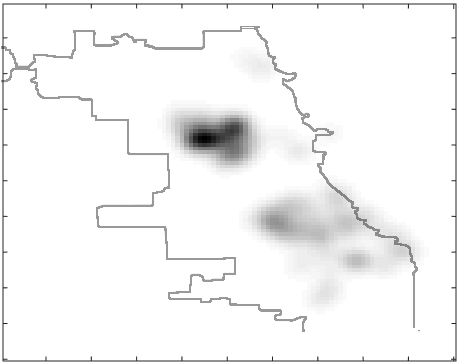
\includegraphics[scale=0.5]{example.png}
 \end{center}
\item Look at gambling crimes from the year 2001 to 2014. 
\item  How has the distribution of gambling crime changed over time?
\item  Generate/turn in a Gaussian kernel density estimate for interference with an officer (crime type 1) in the year 2014.
\end{enumerate}

\section{Extra}

\begin{enumerate}
\item The modeling of salaries above allows for the city of Chicago to theoretically charge people to work for them! What does this say 
about the model? How could we change the model to fix this?
\item Can you think of an analogous issue the kernel density estimation suffers from? Hint: Chicago rests on the perimeter of lake Michigan.
\end{enumerate}


\end{document}
